\section{GinVoice}\label{sec:ginvoice}
In this chapter, we will take a closer look at GinVoice — an open-source Python GTK application that utilizes \LaTeX\ behind the scenes to create invoices.
Additionally, we will examine the provided invoice template and delve into the associated data within the invoice.

\subsection{The Application}
GinVoice has multiple views.
The most common view is the main view, where you can draft multiple invoices simultaneously.
In this view, depicted in figure~\ref{fig:app}, almost all components are visible.
\begin{figure}[!ht]
    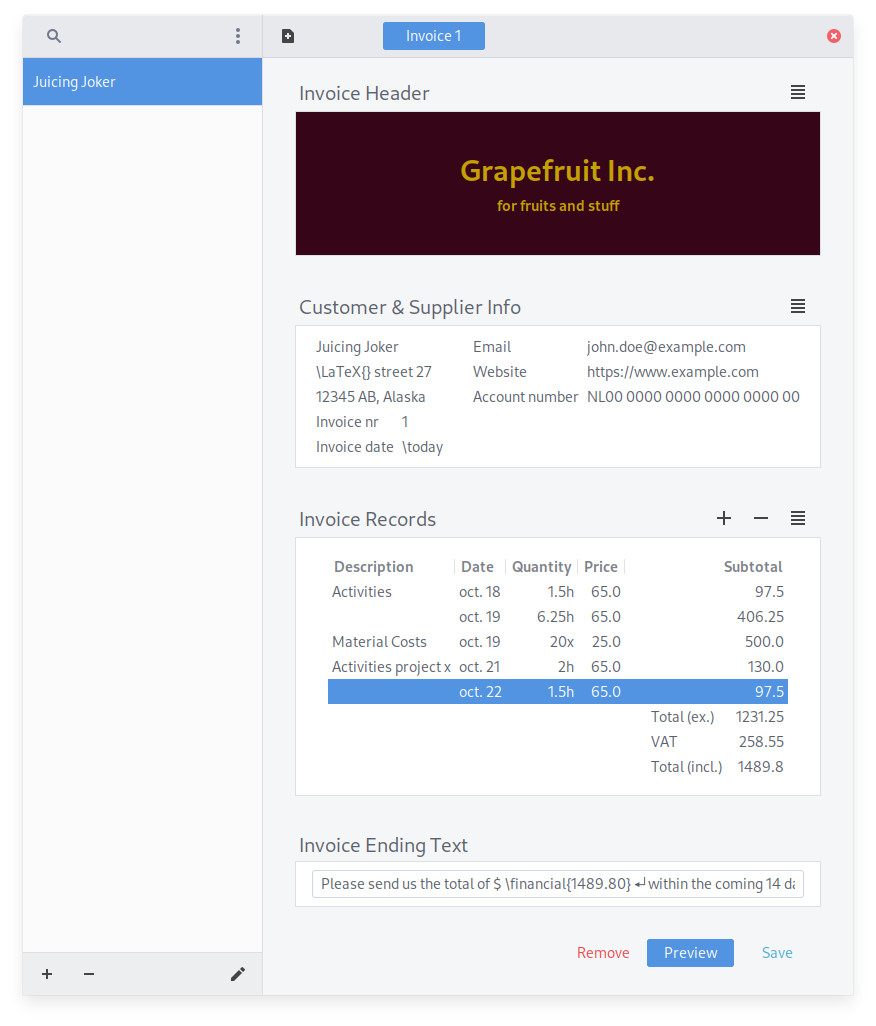
\includegraphics[width=\linewidth]{ginvoice/app.jpg}
    \caption{GinVoice — the application}\label{fig:app}
\end{figure}
You can see the header, information tables, invoice rules, and the closing text included in it. Figure~\ref{fig:app} shows that the input fields are already filled in, and their content does not deviate much when compared to the end result, as seen in figure~\ref{fig:sampleinvoice}. Other application views will be discussed later in this chapter.
\begin{figure}[!ht]
    \centering
    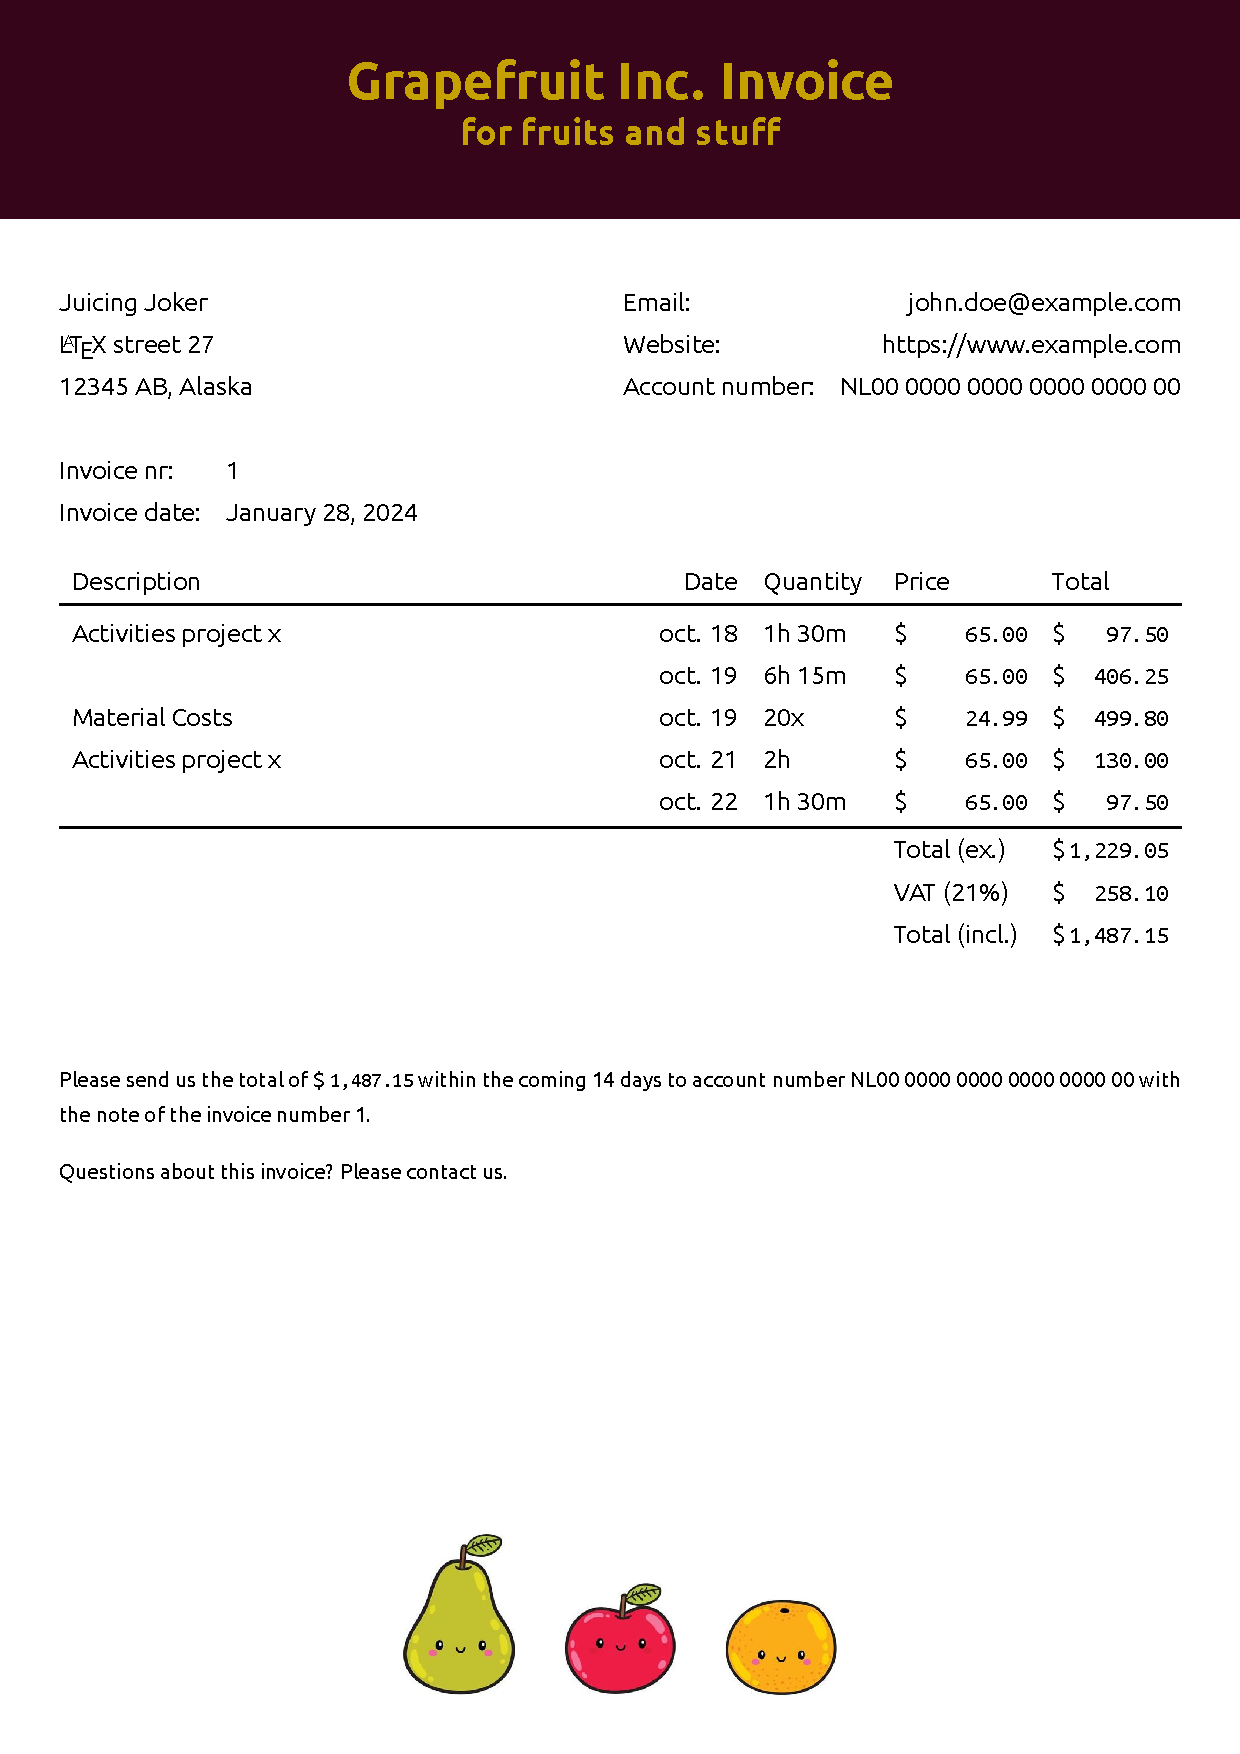
\includegraphics[width=\linewidth]{ginvoice/ginvoice.pdf}
    \caption{Sample invoice generated with GinVoice}
    \label{fig:sampleinvoice}
\end{figure}

\subsection{\LaTeX\ Template}
Below is an example of the code within the \texttt{document} environment:

\lstinputlisting[name=invoice-original,language={[LaTeX]TeX},firstnumber=52,linerange={52-81},numbers=left,xleftmargin=15pt,label={lst:main},caption={\texttt{invoice.tex}}]{ginvoice/invoice-original.tex}

The source code in listing~\ref{lst:main} demonstrates various macros that will be replaced by \pkg{lua-placeholders}, including \cs{title}, \cs{subtitle}, \cs{addressee}, \cs{customerinfo}, \cs{supplierinfo}, \cs{tablefooter}, \cs{tablerecords}, \cs{theending}, and \cs{images}.
Additionally, there are variables such as style-related information and \cs{currency} that will also be handled.

\subsection{Generated \LaTeX\ Files}
It is important to note that GinVoice\cite{ginvoice} currently uses a Python script -- \texttt{generator.py} -- to generate additional \TeX\ files.
These \TeX\ files are then included in the template using \cs{include}, making the necessary macros available.
%However, with the introduction of \pkg{lua-placeholders}, this approach will no longer be necessary.

Starting with the language setting:
\begin{figure}[!ht]
    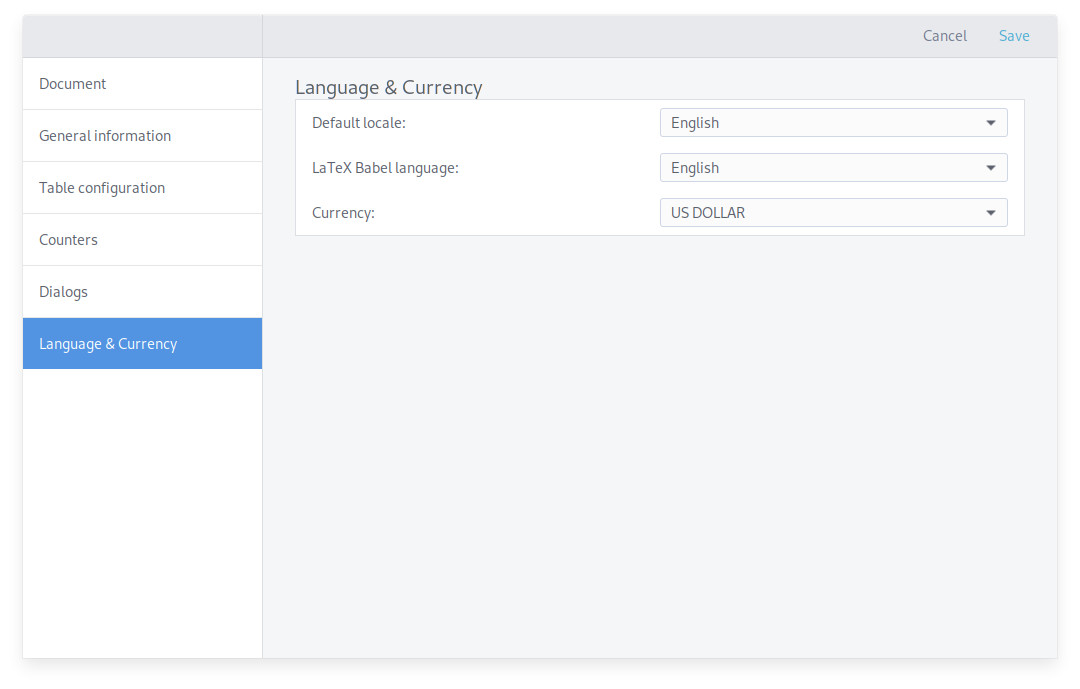
\includegraphics[width=\linewidth]{ginvoice/locale.jpg}
    \caption{Language settings}\label{fig:locale}
\end{figure}
\lstinputlisting[language={[LaTeX]TeX},caption={\texttt{languages.tex}}]{ginvoice/languages.tex}
At the time, I chose to include a separate language setting in the application, as shown in figure~\ref{fig:locale}, so that words within the invoice are neatly hyphenated using \pkg{babel}.

Another aspect within the preamble is setting the document properties. These macros are imported from the generated file \texttt{meta.tex}, whose macros are later used in the \cs{hypersetup}.
\lstinputlisting[language={[LaTeX]TeX},caption={\texttt{meta.tex}}]{ginvoice/meta.tex}
Common macros, such as \cs{title}, are used in multiple places. That is also why the \cs{title} does not need to be in the \texttt{header.tex}.
\lstinputlisting[language={[LaTeX]TeX},caption={\texttt{header.tex}}]{ginvoice/header.tex}
The customer's address is placed in a macro, with the address lines separated by a newline.
\lstinputlisting[language={[LaTeX]TeX},caption={\texttt{addressee.tex}}]{ginvoice/addressee.tex}
This approach would be suitable for a table with a single column or for, say, an \texttt{enumerate} environment.

The customer and supplier information assumes a table environment with two columns.
\lstinputlisting[language={[LaTeX]TeX},caption={\texttt{customer\_info.tex}}]{ginvoice/customer_info.tex}
\lstinputlisting[language={[LaTeX]TeX},caption={\texttt{supplier\_info.tex}}]{ginvoice/supplier_info.tex}
The drawback of this setup is that an ampersand (\&) does not have any function within the context of the macro itself. That would only be the case when working within a \texttt{tabular} environment. Despite most \LaTeX\ editors giving an error for this, strangely enough, this approach still works.

The most significant challenge within the application was making the invoice table configurable.
\begin{figure}[!ht]
    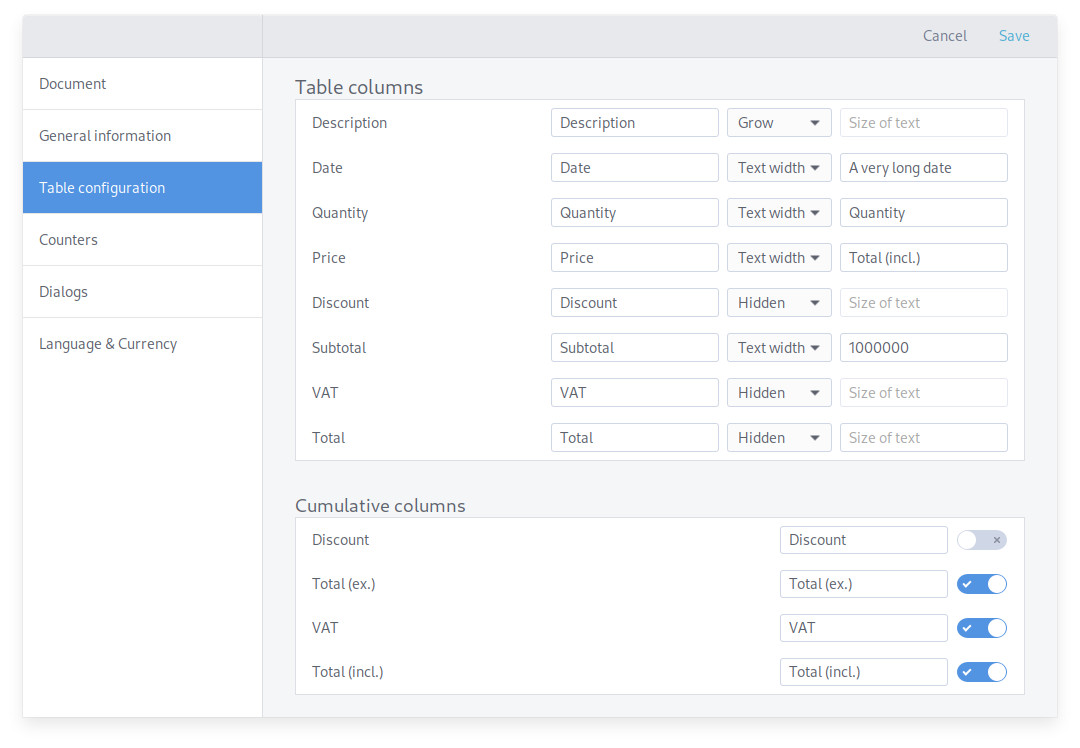
\includegraphics[width=\linewidth]{ginvoice/table-settings.jpg}
    \caption{Table settings}\label{fig:tableconfig}
\end{figure}
For this, there is a separate view, as seen in figure~\ref{fig:tableconfig}.
In the figure, you can see that each column can have a different width, including length of text, maximum available space, or hidden.
This added complexity from the application resulted in a quite complex outcome on the generated \texttt{table.tex} file, as shown in the following code:
\lstinputlisting[language={[LaTeX]TeX},caption={\texttt{table.tex}}]{ginvoice/table.tex}
In addition to the complex column configuration, there are \cs{tablerecords} and \cs{tablefooter}, both similar to, for example, the supplier information.

The last generated file \texttt{footer.tex} defines the remaining missing macros, \cs{theending} and \cs{images}:
\lstinputlisting[language={[LaTeX]TeX},caption={\texttt{footer.tex}}]{ginvoice/footer.tex}
At the time, I chose to store all graphic files somewhere within the GinVoice environment.
I managed to link this to \LaTeX\ by using \cs{graphicspath}.

\subsection{Invoice Data}\label{sec:invoice data}
When looking at all the information coming from GinVoice, with exceptions aside, we end up with the data presented in figure~\ref{fig:classdiagram}.

\begin{figure}[!ht]
    \centering
    \begin{tikzpicture}
    \begin{class}[text width=5cm]{Invoice}{1.75,0}
        \attribute{title : String = Invoice}
        \attribute{subtitle : String}
        \attribute{currency : String = \cs{EUR}}
        \attribute{number : Number}
        \attribute{date : String = \cs{today}}
        \attribute{records : Table}
        \attribute{totals : Table/Object}
        \attribute{ending : String}
    \end{class}
    \begin{class}[text width=3cm]{Supplier}{3.5,-4.75}
        \attribute{email : String}
        \attribute{website : String}
        \attribute{accountnr : String}
    \end{class}
    \begin{class}[text width=3cm]{Client}{0,-4.75}
        \attribute{name : String}
        \attribute{street : String}
        \attribute{postal : String}
        \attribute{place : String}
    \end{class}
    \begin{class}[text width=4cm]{Style}{3,-7.5}
        \attribute{images : List}
        \attribute{main font : String}
        \attribute{mono font : String}
        \attribute{foreground color : String}
        \attribute{background color : String}
        \attribute{\sout{colored table} : Boolean}
    \end{class}
    \draw[umlcd style, diamond-angle 45] ($(Invoice.south west) - (-1.25,0)$) -- ($(Client.north) + (.375,0)$);
    \draw[umlcd style, diamond-angle 45] ($(Invoice.south east) + (-1.25,0)$) -- ($(Supplier.north) + (-.375,0)$);
    \draw[umlcd style, diamond-angle 45] ($(Supplier.south) + (-.375,0)$) -- ($(Style.north) + (.125,0)$);
\end{tikzpicture}

    \caption{Class diagram of the invoice}
    \label{fig:classdiagram}
\end{figure}

For convenience, I have already divided all the information into separate entities, which will correspond to the YAML files, extensively discussed in chapter~\ref{sec:new situation}.
